\documentclass{beamer}
\usepackage{etoolbox}
\usepackage{comment}
\usepackage{graphicx}
\usepackage{dsfont}
\usepackage{amsmath,amssymb}
\usepackage[english]{babel}
\usepackage[svgnames,hyperref]{}
\usepackage{empheq}
\usepackage[many]{tcolorbox}
\usepackage{remreset}
\usepackage{tikz} 
\usetikzlibrary{tikzmark,fit,shapes.geometric}
\usetikzlibrary{tikzmark,calc,arrows,shapes,decorations.pathreplacing}
\tikzset{every picture/.style={remember picture}}
\usepackage{cancel}
\usepackage{booktabs,natbib}
\setbeamercovered{invisible}


\usepackage{dcolumn}


\setbeamertemplate{navigation symbols}{}%remove navigation symbols

\mode<presentation>{}
%% preamble
\title[Essays in Consumption]{Essays in Consumption}
\author{Edmund Crawley}
\date[05/06/2019]{May 6, 2019}

\usetheme{Singapore}


\begin{document}
\newcommand*\circled[1]{\tikz[baseline=(char.base)]{
		\node[shape=circle,draw,inner sep=2pt] (char) {#1};}}
\begin{frame}[plain]
\titlepage
\end{frame}
\setbeamercovered{transparent}
\frame
{
	\frametitle{Overview}
	\setlength{\leftmargini}{2.5cm}
	\begin{itemize}
	\item<1->[Chapter 1]{Time Aggregation in Panel Data on Income and Consumption}
	\item<2->[Chapter 2]{Consumption Heterogeneity: Micro Drivers and Macro Implications}
	\item<3->[Chapter 3]{Monetary Policy with Many Agents}
	\end{itemize}
}
\section{Chapter 1: Time Aggregation}
\frame
{
	\frametitle{Problem}
	Three methods to estimate Marginal Propensity to Consume
	\begin{itemize}
	\item<2-> Natural Experiments $\sim$ 0.2 - 0.7
	\item<3-> Ask people $\sim$ 0.2 - 0.5
	\item<4-> \tikzmark{start}\cite{blundell_consumption_2008} $\sim$ 0.05 \tikzmark{end}
\end{itemize}
	\only<5->{
		\bigskip
	\textbf{Outlier} downward biased due to the \textbf{Time Aggregation Problem}
	
\begin{tikzpicture}[remember picture,overlay]
	\node[draw,line width=2pt,red,ellipse,inner ysep=10pt,fit={(pic cs:start) (pic cs:end)}] {};
	\end{tikzpicture} 
	This paper corrects estimate to be $\sim$ 0.25
}
}
\frame[t]
{
	\frametitle{Key to BPP Identification}
	Income consists of \textit{permanent} and \textit{transitory} shocks\\
	\vspace{1cm}
	$\Delta y_{t+1}=\Delta p_{t+1}+\Delta \varepsilon_{t+1}$ is a \textit{valid instrument} for $\varepsilon_{t}$\tikz[baseline]{\node(transitory){}}\\
	\only<1->{
		\begin{tikzpicture}[remember picture,overlay]
		\node (transitorya)  at ([shift={(-.2,0.1)}]transitory) {};
		\node (transitoryb)  at ([shift={(0.6,0.6)}]transitorya) {};
		\draw[blue,thick,->] (transitorya)  to [in=225,out=45] (transitoryb) node[anchor=south,text = blue] {Transitory shock year $t$};
		\end{tikzpicture}
	}
	\only<2->{
		\begin{itemize}
			\item Negatively correlated with transitory shocks in year $t$
			\begin{center}
				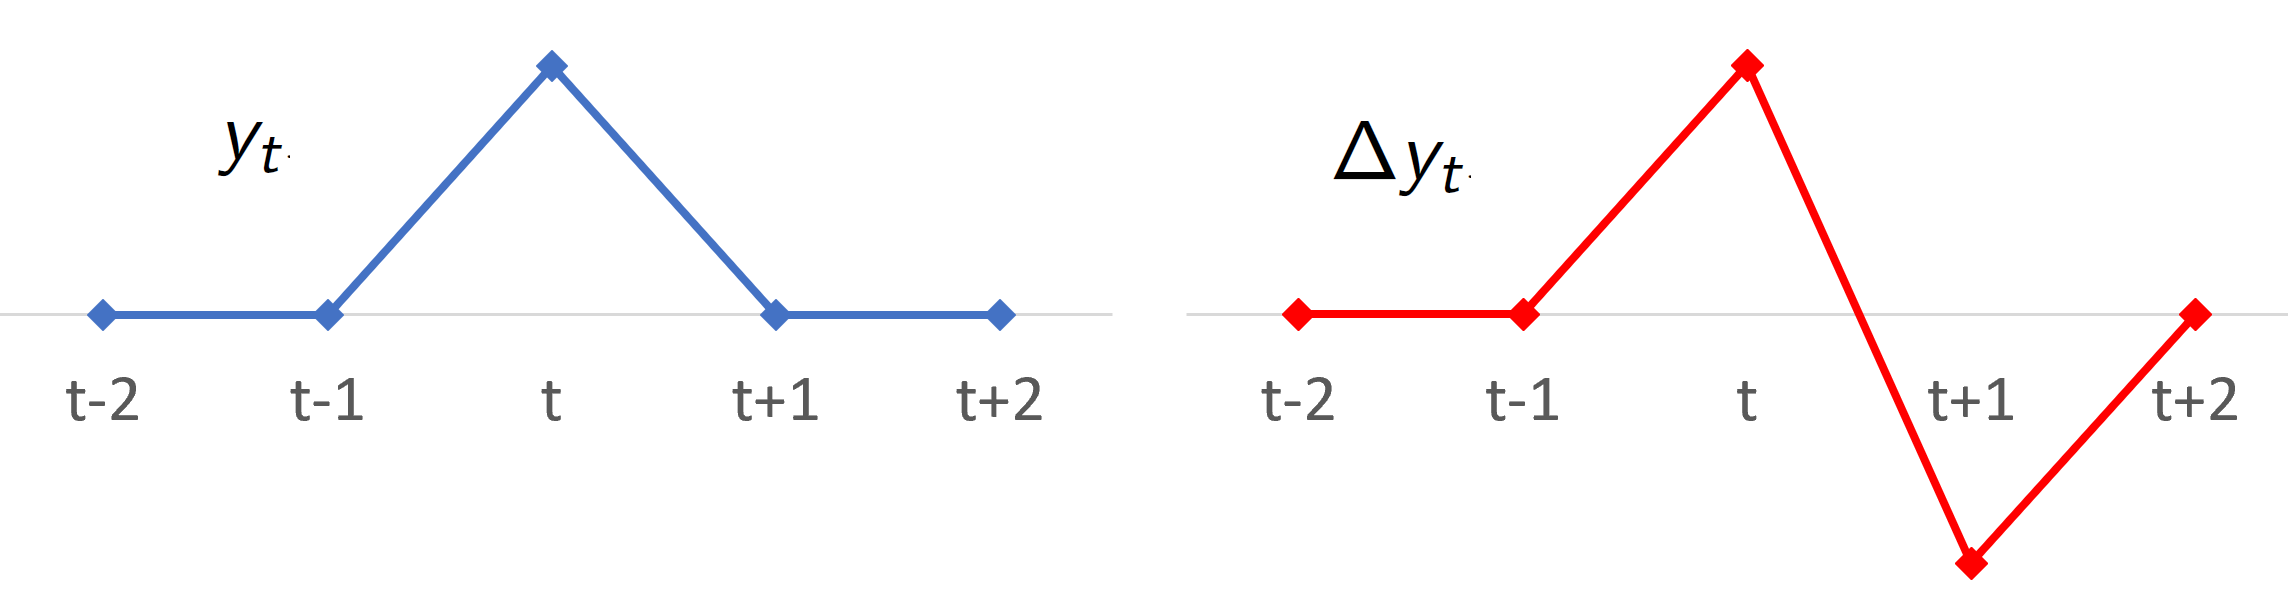
\includegraphics[width=7cm]{./Chapter2/Paper/Slides/SlideFigures/IncGrowthTran.png}
			\end{center}
		\end{itemize}
	}
	\only<3->{
		\begin{itemize}
			\item U\tikzmark{start}ncorrelated with permanent shocks in year \tikzmark{end}$t$
			\begin{center}
				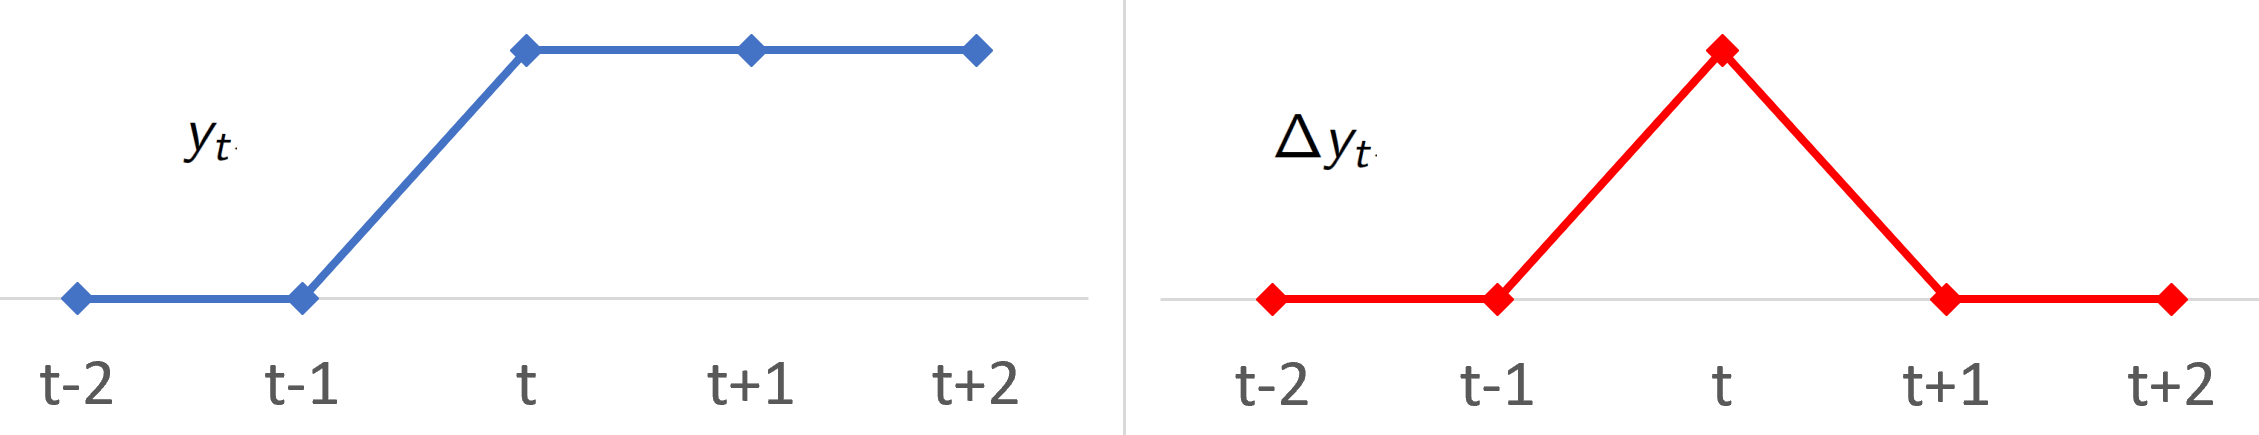
\includegraphics[width=7cm]{./Chapter2/Paper/Slides/SlideFigures/IncGrowthPerm.png}
			\end{center}
		\end{itemize}
	}
	\only<4->{
		
\begin{tikzpicture}[remember picture,overlay]
		\node[draw,line width=2pt,red,ellipse,inner ysep=10pt,fit={(pic cs:start) (pic cs:end)}] {};
		\end{tikzpicture} 
	}
}
\frame
{
	\frametitle{Time Aggregation}
	\setbeamercovered{invisible}
	\begin{columns}
		\column{0.5\linewidth}
		\centering
		\onslide<1->{
			\begin{tikzpicture}
			\node (img1) {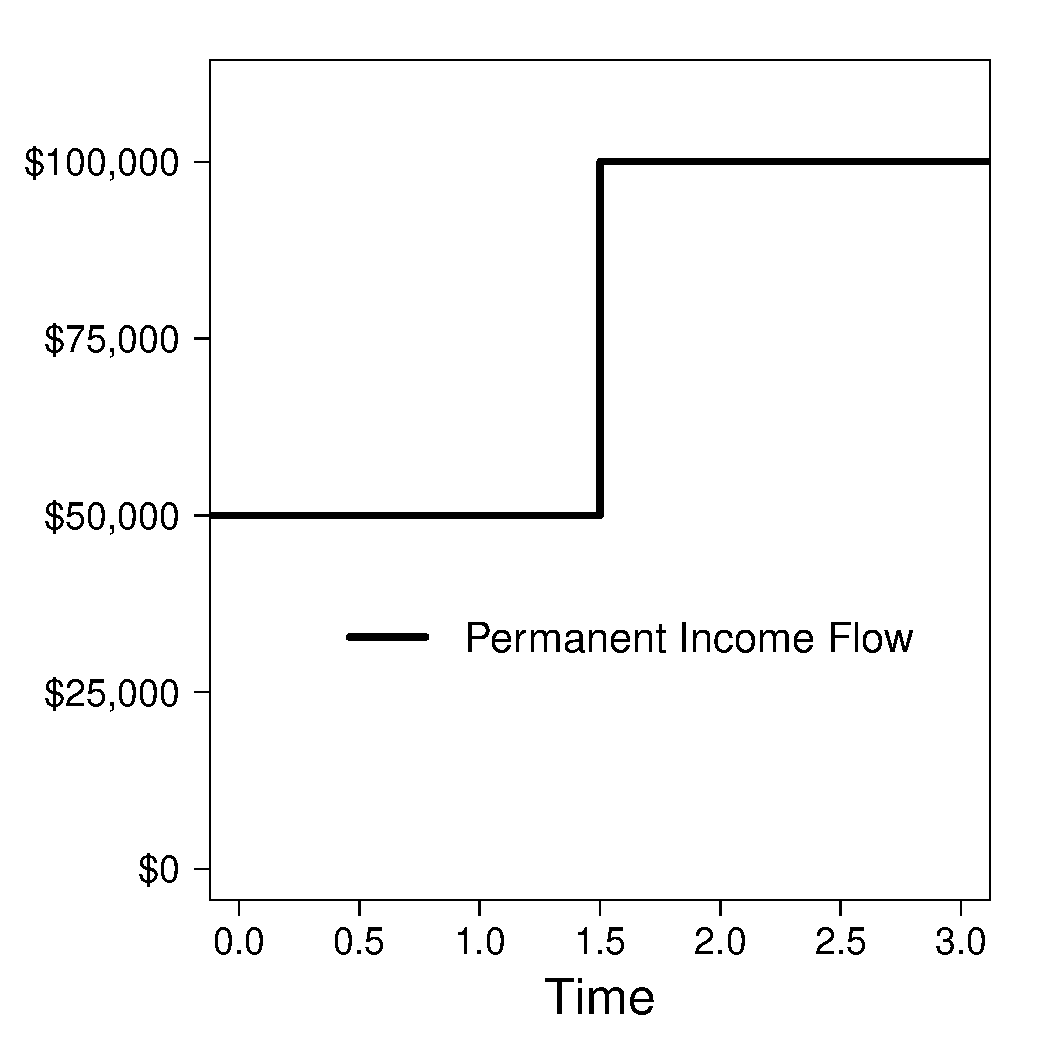
\includegraphics[height=5cm]{./Chapter2/Paper/Figures/TimeAggExample1_slides.pdf}};
			\onslide<2->{
				\node (img2) {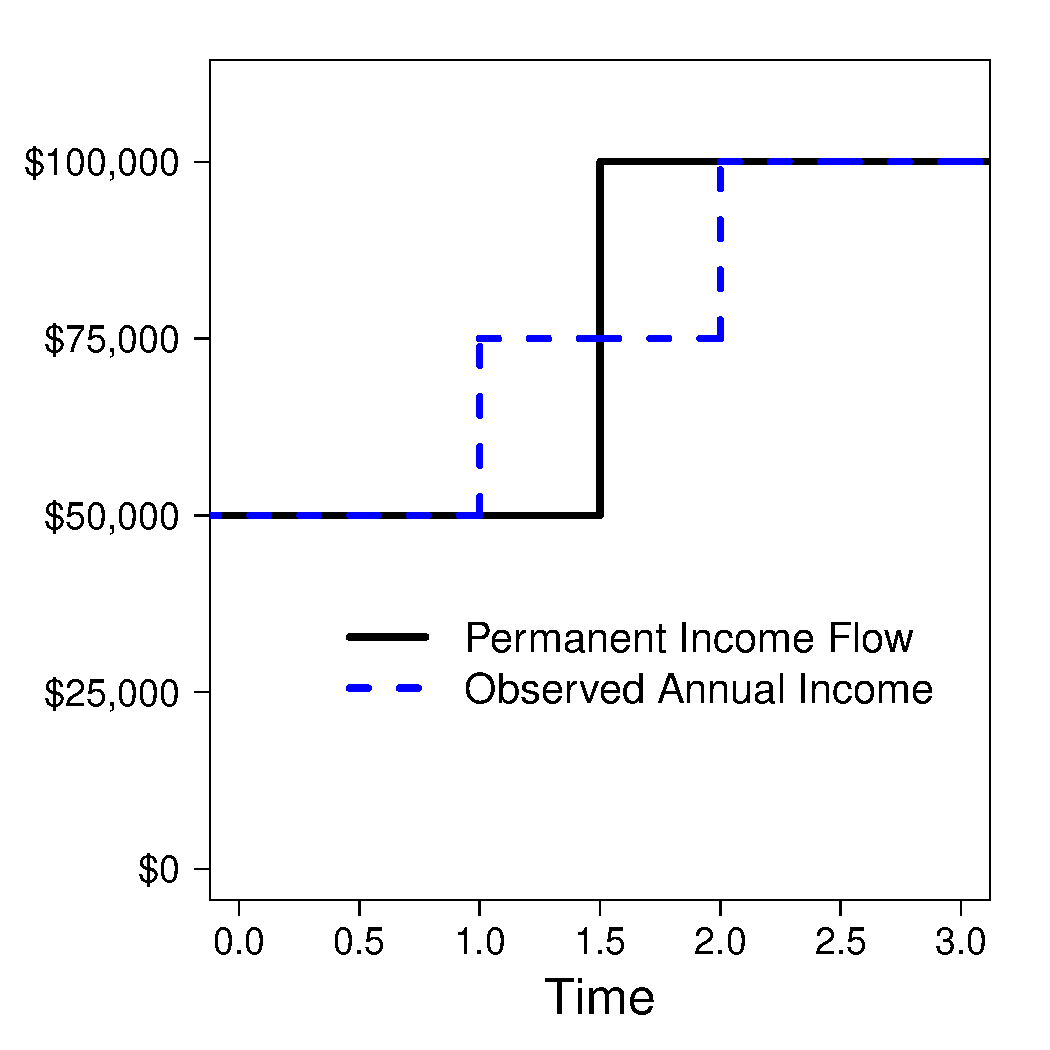
\includegraphics[height=5cm]{./Chapter2/Paper/Figures/TimeAggExample2_slides.pdf}};
			}
			\end{tikzpicture}
		}
		\column{0.5\linewidth}
		\setbeamercovered{transparent}
		\onslide<3->{Observed permanent income growth is \textit{positively} autocorrelated\\
			\bigskip
			BPP misinterprets \textit{positive} permanent income shocks as \textit{negative} transitory shocks\\
			\bigskip
			$\implies$ Thinks negative transitory shocks result in consumption \textit{increasing}
		\end{columns}
	}
	\setbeamercovered{transparent}
	\onslide<4->{If the Permanent Income Hypothesis holds, BPP will estimate the MPC to be -0.6}
}
\frame{
	\frametitle{Results}
	Estimate of consumption: 0.05 $\rightarrow$ 0.24
	\begin{itemize}
		\item Exact Same PSID data
		\item Exact Same Moments of the data
		\item Exact Same Assumptions on consumption behavior\tikz[baseline]{\node(cons_assumptions){}}
	\end{itemize}
	\begin{tikzpicture}[remember picture,overlay]
	\node (cons_assumptions1a)  at ([shift={(-5,-0.0)}]cons_assumptions) {};
	\node (cons_assumptions1b)  at ([shift={(0.5,-1)}]cons_assumptions1a) {};
	\draw[blue,thick,->] (cons_assumptions1a)  to [in=180,out=270] (cons_assumptions1b) node[anchor=west,text = blue] {Adjusted to Continuous Time};
	\end{tikzpicture}
	\\
	\vspace{1.1cm}
	\pause
	BUT: Result is \textit{very} sensitive to short term dynamics of consumption
}
\section{Chapter 2:Consumption Heterogeneity}
\frame
{
	\frametitle{Measuring MPC Heterogeneity}
	\bigskip
	\hspace{1cm} New \textbf{method} addresses bias in previous results  \tikz[baseline]{\node(bias){}}\\
	\bigskip
	\hspace{1cm} New \textbf{data} allows sharp focus on household heterogeneity  \tikz[baseline]{\node(data){}}\\ 
	\only<2->{
		\begin{tikzpicture}[remember picture,overlay]
		\node (bias1a)  at ([shift={(-3.5,0.3)}]bias) {};
		\node (bias1b)  at ([shift={(0,1)}]bias1a) {};
		\draw[blue,thick,->] (bias1a)  to [in=270,out=90] (bias1b) node[anchor=south,text = blue] {\begin{tabular}{l} Time Aggregation Problem\\ Robust to short term dynamics \end{tabular}};
		\end{tikzpicture}
	}
	\only<3->{
		\begin{tikzpicture}[remember picture,overlay]
		\node (data1a)  at ([shift={(-8.2,-0.0)}]data) {};
		\node (data1b)  at ([shift={(0.5,-1)}]data1a) {};
		\draw[blue,thick,->] (data1a)  to [in=180,out=270] (data1b) node[anchor=west,text = blue] {\begin{tabular}{l} Sample size in millions\\ Detailed balance sheet \end{tabular}};
		\end{tikzpicture}
	}
}
\frame
{
	\frametitle{Why Do We Care? (as macroeconomists)}
	1) Heterogenous agent models have testable micro behavior \tikz[baseline]{\node(micro){}}\\
	\bigskip
	2) Quantify Macro Implications \tikz[baseline]{\node(macro){}}
	\only<2->{
		\begin{tikzpicture}[remember picture,overlay]
		\node (micro1a)  at ([shift={(-2.2,0.3)}]micro) {};
		\node (micro1b)  at ([shift={(-1,0.8)}]micro1a) {};
		\draw[blue,thick,->] (micro1a)  to [in=270,out=90] (micro1b) node[anchor=south,text = blue] {\begin{tabular}{l} e.g. Consumption smoothing requires liquid wealth  \end{tabular}};
		\end{tikzpicture}
	}
	\only<3->{
		\begin{tikzpicture}[remember picture,overlay]
		\node (macro1a)  at ([shift={(-2.8,0.0)}]macro) {};
		\node (macro1b)  at ([shift={(-0.0,-0.8)}]macro1a) {};
		\draw[blue,thick,->] (macro1a)  to [in=90,out=270] (macro1b) node[anchor=north,text = blue] {\begin{tabular}{l} e.g. Redistribution in Monetary Policy  \end{tabular}};
		\end{tikzpicture}
	}
}
\frame
{
	\frametitle{What do we find? (Liquid Wealth)}
	Low Liquid Wealth Households:
	\begin{itemize}
		\item Hand-to-Mouth
		\item Spend 85 cents out of every marginal dollar, both transitory and permanent
	\end{itemize}
	\bigskip
	\pause
	High Liquid Wealth Households: 
	\begin{itemize}
		\item Large Response to Transitory Shocks (25 cents per dollar)
		\item Small Response to Permanent Shocks (60 cents per dollar)
	\end{itemize}
	relative to Permanent Income Hypothesis or Buffer-Stock models
}
\frame[t]
{
	\frametitle{What do we find? (Redistribution in Monetary Policy)}
	\only<1>{
		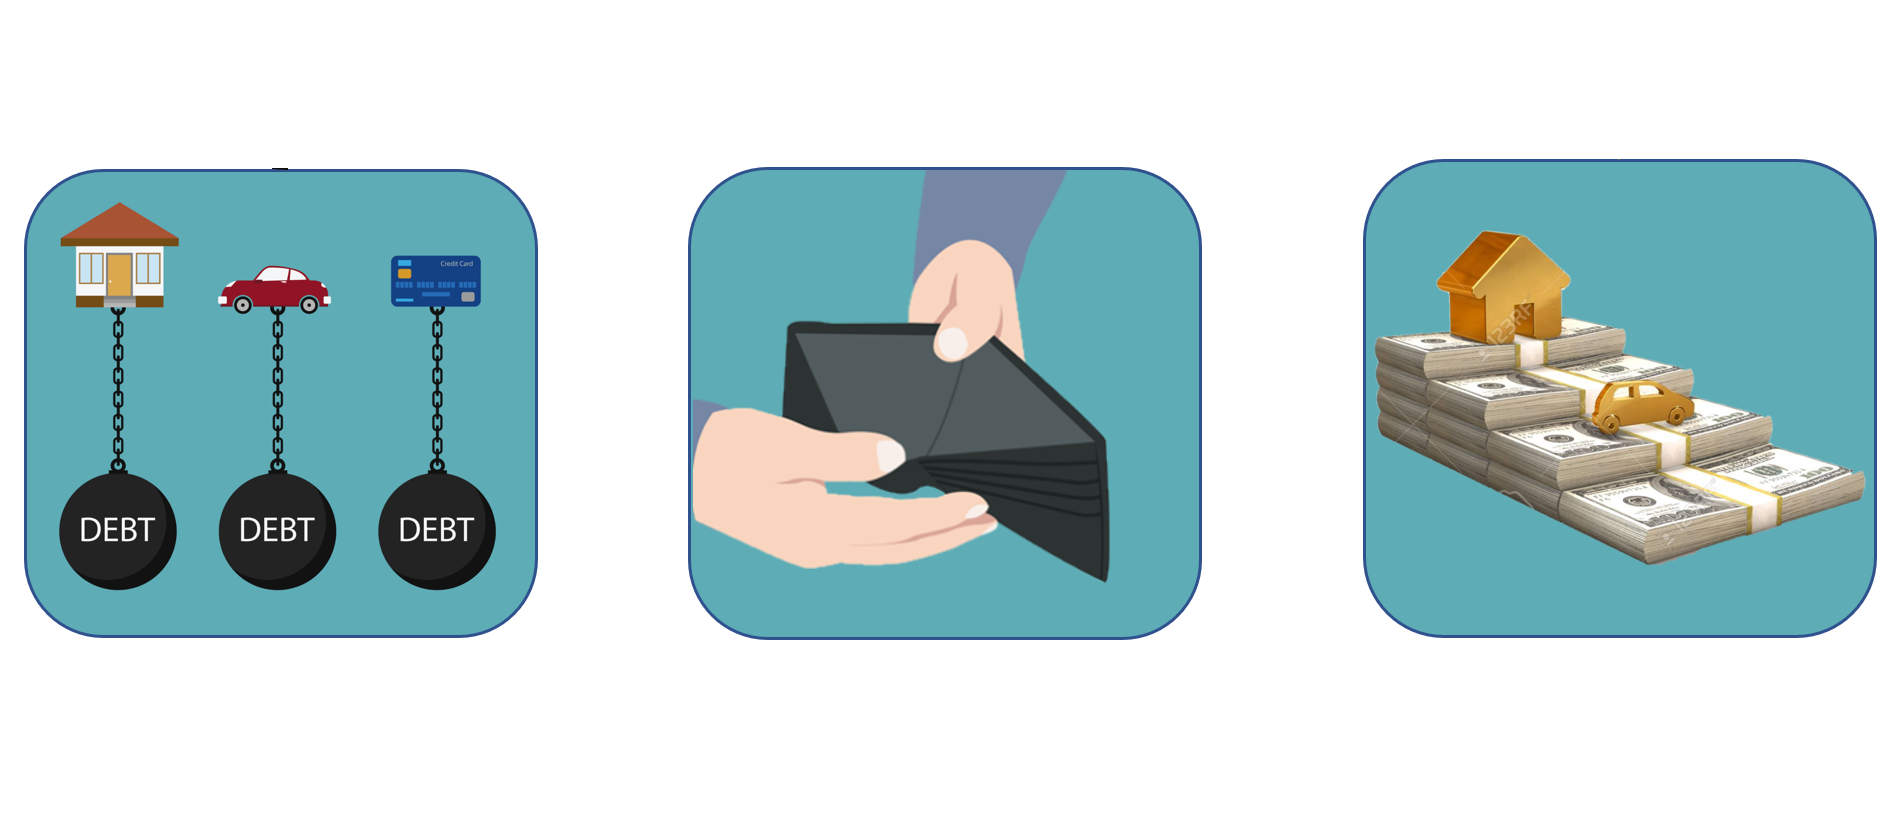
\includegraphics[width=11cm]{./Chapter2/Paper/Slides/SlideFigures/IRE_Big1.png}
	}
	\only<2>{
		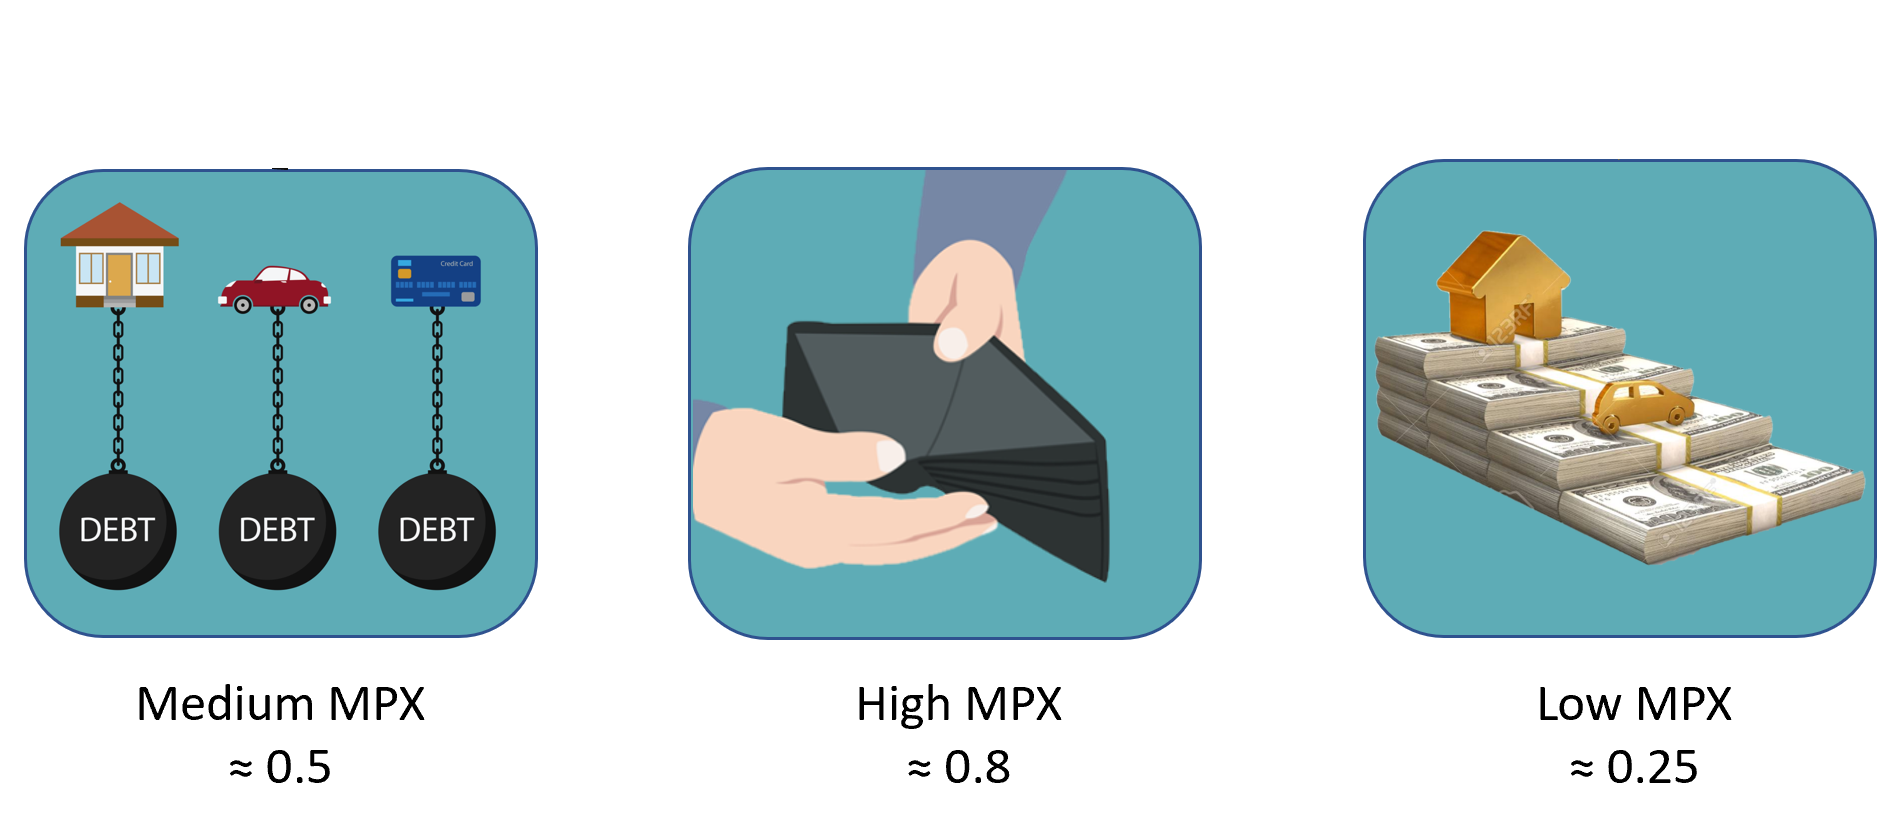
\includegraphics[width=11cm]{./Chapter2/Paper/Slides/SlideFigures/IRE_Big2.png}
		\\[0.7cm]
		MPX: Marginal Propensity to eXpend (includes durables)
	}
	\only<3->{
		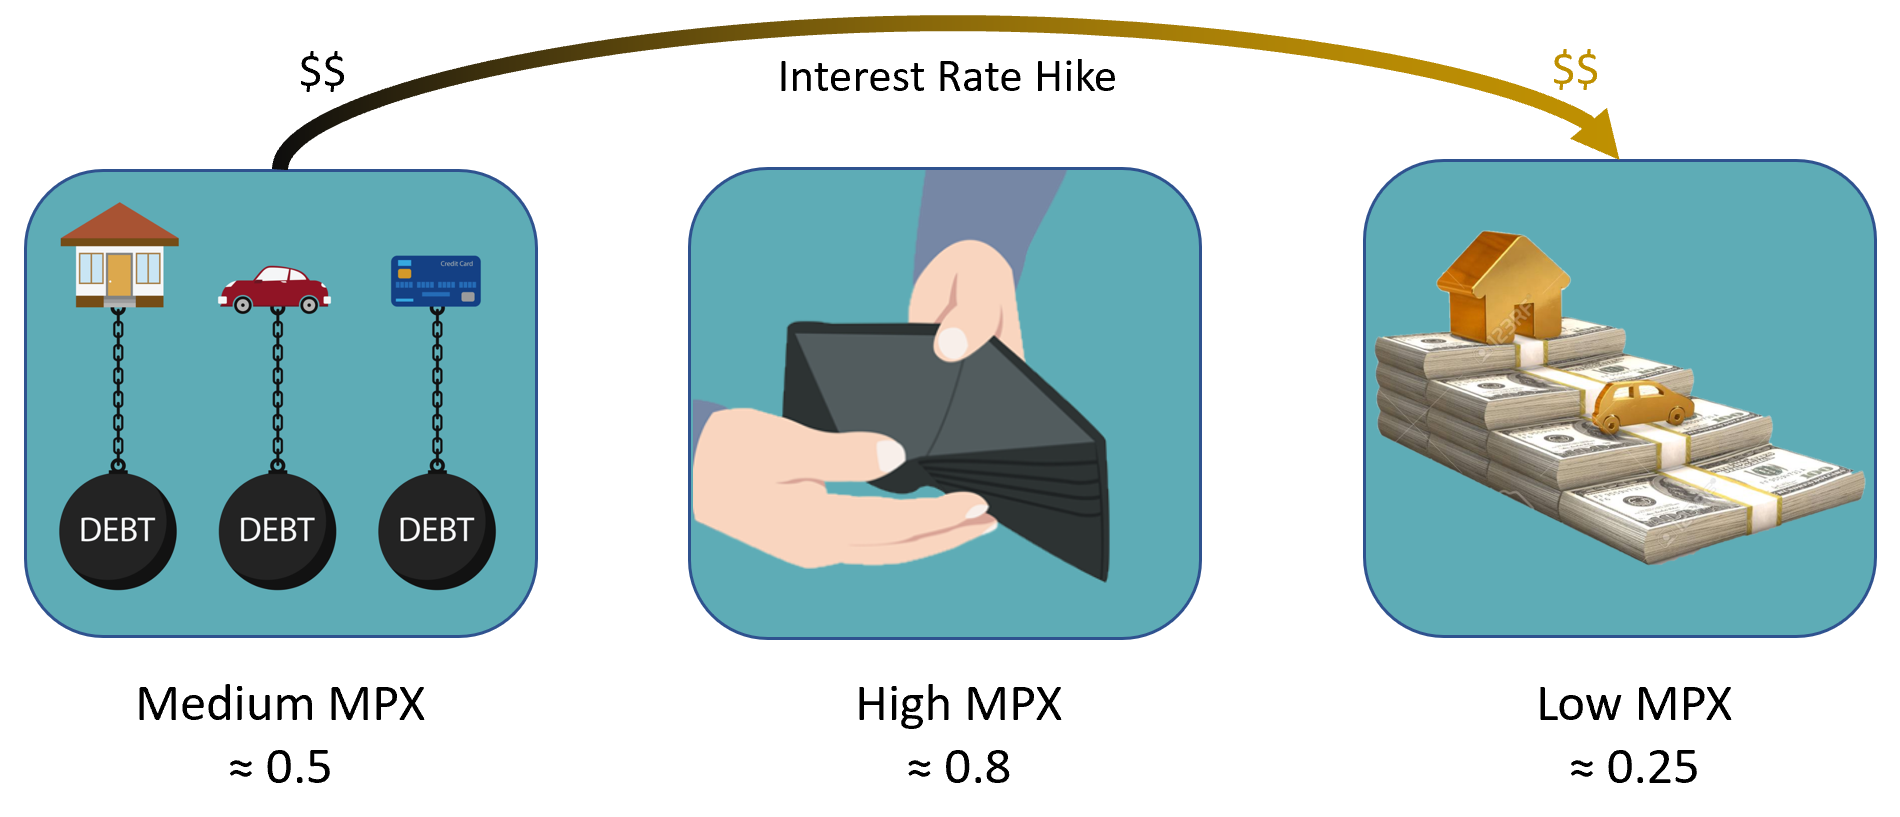
\includegraphics[width=11cm]{./Chapter2/Paper/Slides/SlideFigures/IRE_Big3.png} \tikz[baseline]{\node(ire){}}
	}
	\only<3>{
		\begin{tikzpicture}[remember picture,overlay]
		\node (ire1a)  at ([shift={(1.3,0.3)}]ire) {};
		\node (ire1b)  at ([shift={(-0.4,-0.4)}]ire1a) {};
		\draw[blue,thick,->] (ire1a)  to [in=45,out=225] (ire1b) node[anchor=north,text = blue] {\begin{tabular}{l} Decrease spending \\ a \textit{lot}  \end{tabular}};
		\node (ire1c)  at ([shift={(9.5,0.3)}]ire) {};
		\node (ire1d)  at ([shift={(0.4,-0.4)}]ire1c) {};
		\draw[blue,thick,->] (ire1c)  to [in=135,out=315] (ire1d) node[anchor=north,text = blue] {\begin{tabular}{r} Increase spending \\ a \textit{little}  \end{tabular}};
		\end{tikzpicture}
	}
	\only<4->{
		\vspace{-.5cm}
		\begin{align*}
		\text{1yr rate }&\uparrow \ 1\% \\
		\tikz[baseline]{\node(aggregate){}} \textit{Aggregate}\text{ Spending }&\downarrow \ 26 \text{ basis points}
		\end{align*}
		\begin{tikzpicture}[remember picture,overlay]
		\node (aggregatea)  at ([shift={(1.5,-0.1)}]aggregate) {};
		\node (aggregateb)  at ([shift={(-0.4,-0.4)}]aggregatea) {};
		\draw[blue,thick,->] (aggregatea)  to [in=45,out=225] (aggregateb) node[anchor=north,text = blue] {Through this redistribution channel \textit{alone}};
		\end{tikzpicture}
	}
}
\section{Chapter 3: Monetary Policy with Many Agents}
\frame
{
	\frametitle{How Does Heterogeneity Effect Monetary Policy Transmission?}
		\setlength{\leftmargini}{2.5cm}
	\begin{itemize}
		\item<1->[Chapter 2]{Interest Rate Exposure is key \textit{empirically}}
		\item<2->[This Chapter]{What drives transmission in New Keynesian models with heterogeneity?}
		\item<2->[]{Can we apply \cite{auclert_monetary_2017} to these models?}
	\end{itemize}
}
\frame
{
	\frametitle{Two Agent New Keynesian Model (TANK)}
	Ricardian Households
	\begin{itemize}
		\item Behave as Representative Agent NK model
	\end{itemize}
	Keynesian Households
	\begin{itemize}
	\item Live hand-to-mouth
	\item Only labor income
	\item Can borrow a fixed fraction of steady-state income
	\end{itemize}
}
\frame{
		\frametitle{Monetary Policy Transmission with No Debt}
		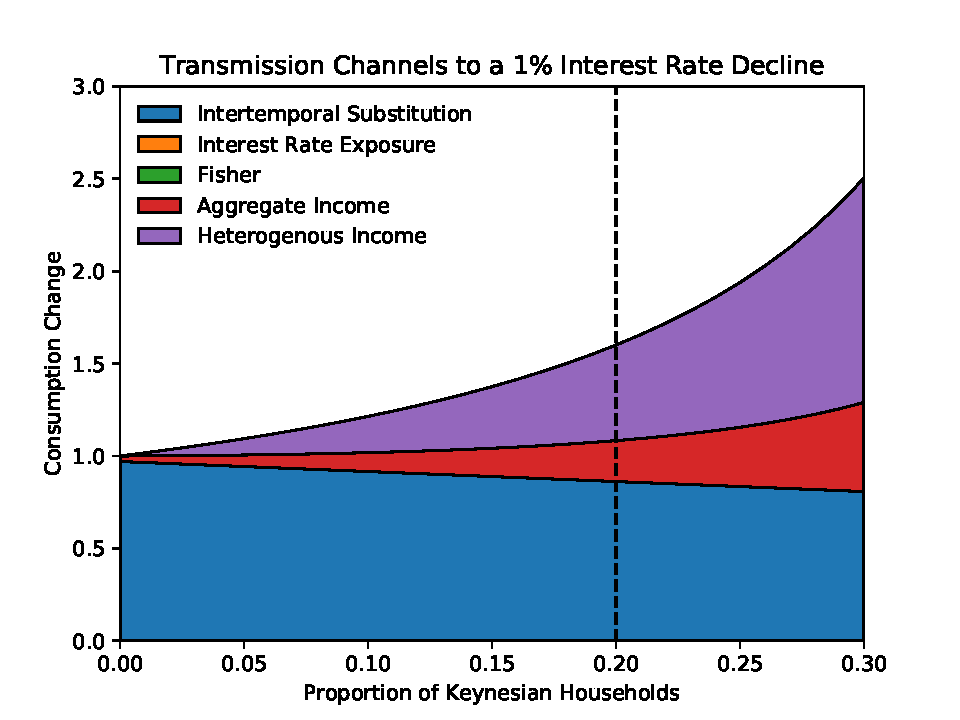
\includegraphics[scale=0.6]{./Chapter3/Python/DoloCode/Figures/ProportionKeynesian_sigma1.pdf}
}
\frame{
	\frametitle{Monetary Policy Transmission with Debt}
	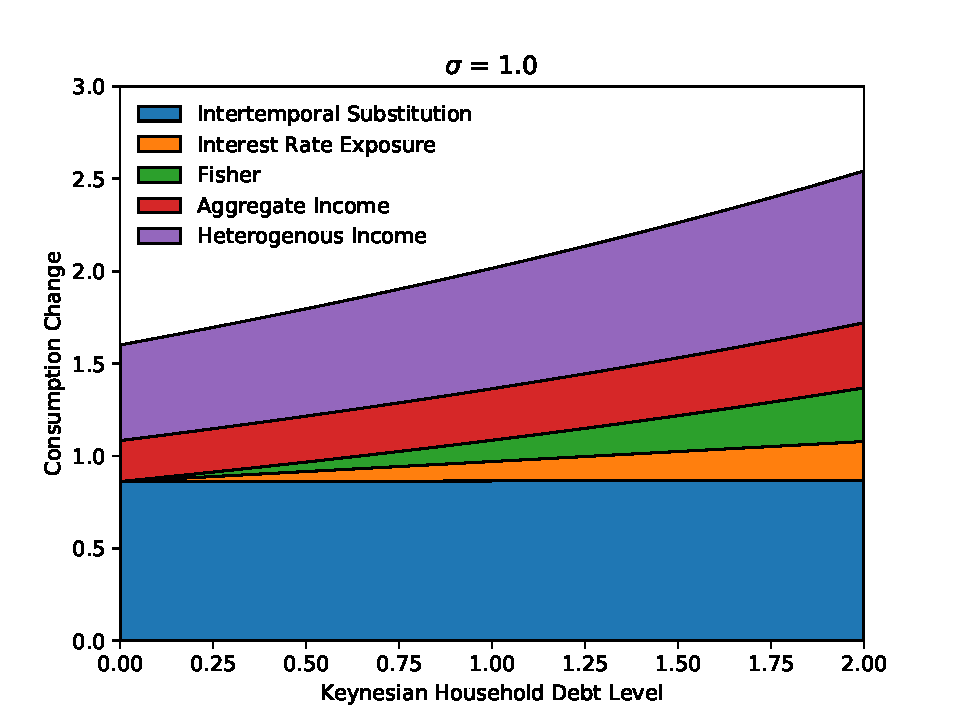
\includegraphics[scale=0.6]{./Chapter3/Python/DoloCode/Figures/KeynesianDebt_sigma1.pdf}
}
\frame{
	\frametitle{Appicability of \cite{auclert_monetary_2017}}
	Capital
	\begin{itemize}
		\item Shocks become persistent
		\item Reasonable adjustment costs reduce persistence
	\end{itemize}
	\pause
	Heterogeneous Agent New Keynesian (HANK) model
	\begin{itemize}
		\item Change is wealth distribution induces little persistence
		\item GHH preferences are a big problem
	\end{itemize}
}
\frame{
Thank You!
}
\bibliographystyle{econometrica}
\newsavebox\mytempbib
\savebox\mytempbib{\parbox{\textwidth}{\bibliography{AllPapers}}}


\end{document}

